\chapter{Analisis}
\label{chap:analisis}
Pada bab ini dijelaskan mengenai analisis aplikasi ekstraksi fitur domain waktu/frekuensi untuk data akselerometer di WSN, analisis proses ekstraksi fitur domain waktu/frekuensi untuk data akselerometer, dan analisis algoritma ekstraksi fitur domain waktu/frekuensi.

\section{Analisis Aplikasi Ekstraksi Fitur Domain Waktu/Frekuensi Untuk Data Akselerometer di WSN}
Berdasarkan latar belakang pada Bab \ref{chap:intro} dan pembahasan landasan teori pada Bab \ref{chap:teori}, penelitian ini akan membangun aplikasi ekstraksi fitur domain waktu/frekuensi pada data akselerometer di sensor node WSN. Untuk membangun aplikasi ini akan dibuat 3 program, yaitu program yang akan berjalan di sensor node dan melakukan ekstraksi fitur, program yang akan berjalan di sensor node sebagai {\it base station} untuk menerima hasil ekstraksi fitur, dan program yang akan berjalan pada komputer pengguna dalam menampilkan hasil ekstraksi fitur. 

Pada subbab selanjutnya akan dijelaskan mengenai analisis topologi, arsitektur, akselerometer, fungsi aplikasi, dan kelas untuk aplikasi ini.

\subsection{Analisis Topologi dan Arsitektur WSN} \label{subsec:analisisTopArs}
Berdasarkan pembahasan Subbab \ref{subsec:topologiWSN} mengenai topologi dan Subbab \ref{subsec:arch} mengenai arsitektur WSN, topologi WSN pada aplikasi ini dapat menggunakan WSN berarsitektur {\it flat} dengan topologi {\it star} atau {\it tree}. WSN dengan Arsitektur {\it flat} dengan seluruh sensor node memiliki tugas yang sama sangat cocok dengan penelitian ini yang hanya melakukan ekstraksi fitur data akselerometer. WSN dengan topologi {\it star} dan {\it tree} juga cocok dengan penelitian ini karena telah mencakup semua tipe komunikasi WSN. Topologi {\it star} memiliki komunikasi yang selalu {\it single-hop} dan {\it sink} sebagai {\it central communication}(Gambar~\ref{fig:star_flat_single}). Topologi {\it tree} dapat memiliki komunikasi {\it single-hop} atau {\it multi-hop} dan {\it sink} sebagai {\it root} dari {\it tree}(Gambar~\ref{fig:tree_flat_multi}).    

		\begin{figure}[H]
			\centering  
			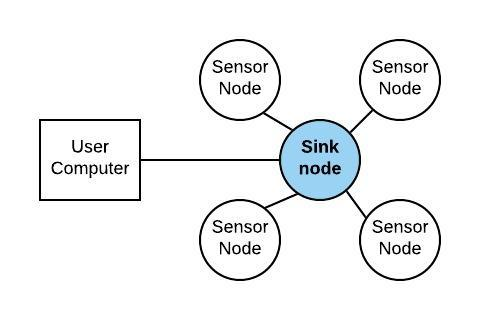
\includegraphics[scale=0.8]{star_flat_single}  
			\caption[WSN dengan topologi {\it star} dengan komunikasi {\it single-hop}]{WSN dengan topologi {\it star} dan komunikasi {\it single-hop}} 
			\label{fig:star_flat_single} 
		\end{figure} 
		
		\begin{figure}[H]
			\centering  
			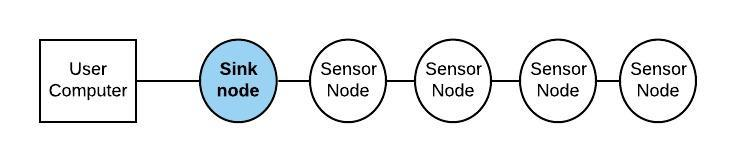
\includegraphics[scale=0.8]{tree_flat_multi}  
			\caption[WSN dengan topologi {\it tree} dengan komunikasi {\it single-hop} dan {\it multi-hop}]{WSN dengan topologi {\it tree} dengan komunikasi {\it single-hop} dan {\it multi-hop} }
			\label{fig:tree_flat_multi} 
		\end{figure} 

\subsection{Analisis Akselerometer}
\label{subsec:akselerometer}
Akselerometer yang digunakan pada penelitian ini adalah akselerometer ADXL345 dari sensor node Preon32 (Subbab \ref{subsubsec:specPreon32}). Jenis dari akselerometer ini adalah {\it three-axis} dan {\it absolute accelerometer} yang telah dibahas pada Subbab \ref{sec:aks}. Hasil pengukuran dari akselerometer dikonversi ke dalam satuan gravitasi ($g$) dan diubah ke dalam satuan akselerasi ($m/s^2$). Pengubahan satuan ini dilakukan hanya untuk mempermudah visualisasi dari hasil pengukuran. Pengukuran akselerometer
yang divisualisasikan adalah amplitudo dari akselerasi. Dari visualisasi pengukuran ini dapat dilihat fluktuasi dari akselerasi yang terukur oleh akselerometer. 

\subsection{Analisis Fungsi Aplikasi}
\label{subsec:analisisFungsi}
Fungsi utama dari aplikasi ini ada pada program yang dijalankan pada komputer pengguna. Tujuan Fungsi ini mengatur interaksi komputer pengguna, {\it base station}, dan sensor node. Dengan fungsi utama ini pengguna hanya perlu mengoperasikan aplikasi ini di komputer dan dapat menerima data hasilnya di komputer. Berikut fungsi - fungsi tersebut.
\begin{enumerate}
\item Memeriksa sensor node yang aktif 
\item Menyamakan waktu semua sensor node
\item Memberikan perintah {\it sense} ke sensor node 
\item Memberikan perintah berhenti / {\it stop sensing} ke sensor node
\item Menyimpan hasil ekstraksi fitur dari {\it sensing} sensor node
\item Menampilkan hasil ekstraksi fitur dari {\it sensing} sensor node
\end{enumerate}

Fungsi memeriksa sensor node yang aktif diperlukan oleh pengguna untuk memastikan sensor node pada WSN sedang aktif. Jika terdapat sensor node yang tidak aktif pengguna dapat melakukan perbaikkan dan konfigurasi kembali WSN tersebut.

Fungsi menyamakan waktu semua sensor node diperlukan karena memory di sensor node yang bersifat {\it volatile} (\ref{subsec:sensorNode}). Jika sensor node mati maka waktu yang ada pada sensor node adalah waktu terakhir sebelum sensor node itu mati sehingga diperlukan penyamaan waktu kembali.

Fungsi memberikan perintah {\it sense} ke sensor node digunakan untuk memulai {\it sensing} getaran pada setiap sensor node dengan akselerometer. Setiap hasil pengukuran tersebut akan langsung diekstraksi fitur dan dikirimkan ke {\it sink} bersama waktu saat {\it sensing}.

Fungsi memberikan perintah berhenti {\it sensing} ke sensor node digunakan untuk memberhentikan perintah {\it sensing} getaran pada sensor node. 

Fungsi menampilkan hasil ekstraksi fitur dari {\it sensing} sensor node dibutuhkan untuk perangkat lunak dapat menyimpan hasil ekstraksi fitur dalam berupa file dan divisualisasikan dalam bentuk grafik.  

Fungsi - fungsi tersebut hanya dapat digunakan di program yang berjalan di komputer pengguna. Program ini membantu pengguna untuk dapat berinteraksi dengan {\it base station} dan sensor node. Interaksi dapat dilihat pada diagram {\it use case} (Gambar~\ref{fig:UseCase}) dan tabel skenario.



\begin{figure} [H]
	\centering  
	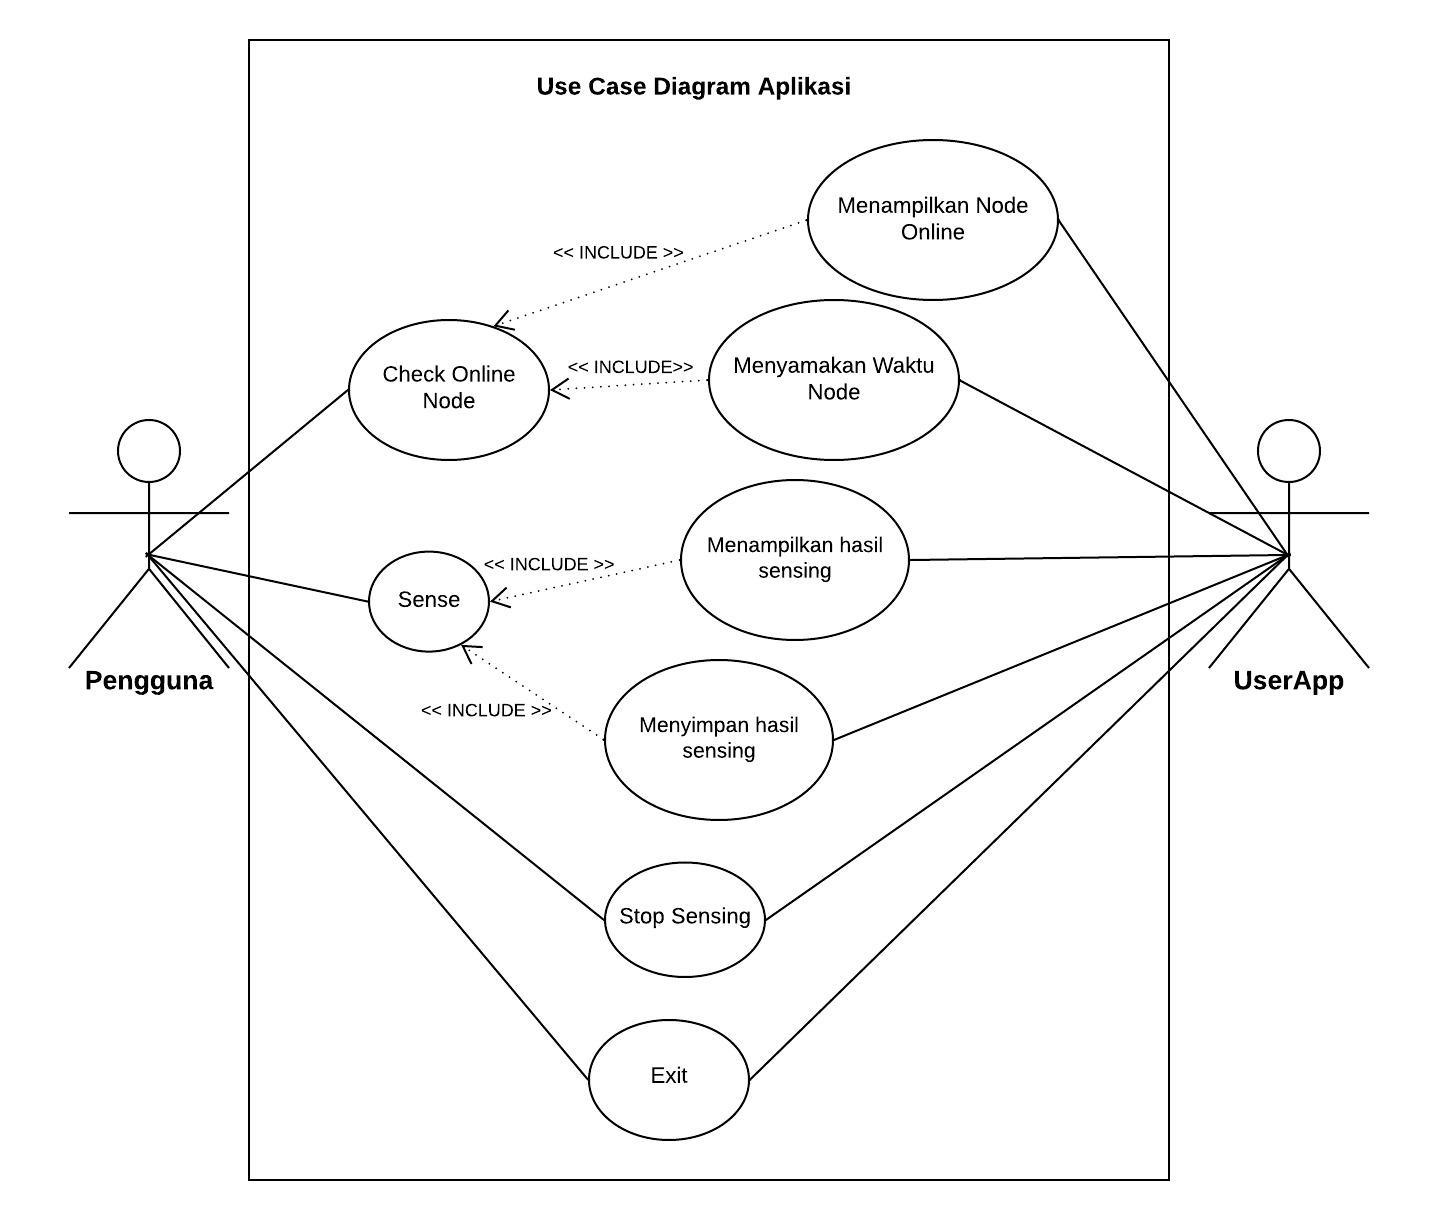
\includegraphics[scale=0.8]{UseCase}  
	\caption[ Diagram {\it use case} Aplikasi Ekstraksi Fitur Domain Waktu/Frekuensi Untuk Data Akselerometer di WSN]{Diagram {\it use case} Aplikasi Ekstraksi Fitur Domain Waktu/Frekuensi Untuk Data Akselerometer di WSN} 
	\label{fig:UseCase} 
\end{figure} 

\begin{table}[H]
    \centering
    \caption{Tabel Skenario Memeriksa sensor node yang aktif / Check Online Node.}
    \begin{tabular}{|p{3cm}|p{10cm}|}
    \hline
        Nama & Memeriksa sensor node yang aktif / Check Online Node\\
    \hline 
    \hline
        Deskripsi & Memeriksa sensor node - sensor node yang aktif dan menyamakan waktu sensor node dengan waktu yang ada pada komputer pengguna. \\
    \hline
        Aktor & Pengguna dan UserApp\\
    \hline
        Pre-kondisi & Aplikasi baru dibuka oleh pengguna. \\
    \hline
        Alur Skenario Utama & 
        \begin{enumerate}
            \item Sistem menjalankan aplikasi.
            \item Pengguna memasukkan total sensor node yang dipakai.
            \item Sistem menampilkan option - option fungsi yang dapat dipilih oleh pengguna.
            \item Pengguna memilih option "Check Online Node".
            \item Sistem menampilkan sensor node dan base station yang online bersama dengan waktu setiap sensor node. 
        \end{enumerate}\\
    \hline
    \end{tabular}
    \label{tab:skenario1}
\end{table}

\begin{table}[H]
    \centering
    \caption{Tabel Skenario Memberikan perintah sense ke sensor node}
    \begin{tabular}{|p{3cm}|p{10cm}|}
    \hline
        Nama & Memberikan perintah sense ke sensor node / Sense\\
    \hline 
    \hline
        Deskripsi & Memberikan perintah sense ke setiap sensor node dan hasil sense dari setiap sensor node yang aktif akan disimpan dan ditampilkan. \\
    \hline
        Aktor & Pengguna dan UserApp\\
    \hline
        Pre-kondisi & Aplikasi sudah berjalan dan fungsi "Check Online Node" sudah digunakan. \\
    \hline
        Alur Skenario Utama & 
         \begin{enumerate}
            \item Sistem menampilkan option - option fungsi yang dapat dipilih oleh pengguna.
            \item Pengguna memilih option "Sense".
            \item Sistem menampilkan hasil sense dan ekstrasi fitur dari setiap sensor node dan menyimpan hasil sense dari setiap node
        \end{enumerate}\\
    \hline
    \end{tabular}
    \label{tab:skenario2}
\end{table}

\begin{table}[H]
    \centering
    \caption{Tabel Skenario Memberikan perintah berhenti sense / Stop Sensing}
    \begin{tabular}{|p{3cm}|p{10cm}|}
    \hline
        Nama & Memberikan perintah berhenti sense / Stop Sensing\\
    \hline 
    \hline
        Deskripsi & Memberikan perintah berhenti sense / Stop Sensing \\
    \hline
        Aktor & Pengguna dan UserApp\\
    \hline
        Pre-kondisi & Aplikasi sudah berjalan dan fungsi "Sense" sudah digunakan. \\
    \hline
        Alur Skenario Utama & 
         \begin{enumerate}
            \item Sistem menampilkan option - option fungsi yang dapat dipilih oleh pengguna.
            \item Pengguna memilih option "Stop Sensing"
            \item Sistem memberhentikan {\it sensing}
            \item Sistem menutup grafik visualisasi.
            \item Sistem menampilkan pesan "Stop Sensing Done". 
        \end{enumerate}\\
    \hline
    \end{tabular}
    \label{tab:skenario3}
\end{table}

\begin{table}[H]
    \centering
    \caption{Tabel Skenario Exit}
    \begin{tabular}{|p{3cm}|p{10cm}|}
    \hline
        Nama & Exit\\
    \hline 
    \hline
        Deskripsi & Memberikan perintah "Exit" untuk basestation dan seluruh sensor node\\
    \hline
        Aktor & Pengguna dan UserApp\\
    \hline
        Pre-kondisi & Aplikasi sudah berjalan. \\
    \hline
        Alur Skenario Utama & 
         \begin{enumerate}
            \item Sistem menampilkan option - option fungsi yang dapat dipilih oleh pengguna.
            \item Pengguna memilih option "Exit"
            \item Sistem menampilkan pesan "program terminated".
            \item Program berhenti. 
        \end{enumerate}\\
    \hline
    \end{tabular}
    \label{tab:skenario4}
\end{table}

\newpage
\subsection{Analisis Kelas}
\label{subsec:analisisKelas}
Pembuatan aplikasi ini menggunakan Eclipse IDE dan SandBox untuk sensor node Preon32 dari Virtenio. Berdasarkan analisis fungsi pada Subbab \ref{subsec:analisisFungsi} maka dibuat diagram kelas sederhana untuk aplikasi ini.
 Berikut diagram kelas sederhana yang dibutuhkan untuk aplikasi ini.

\begin{figure} [H]
	\centering  
	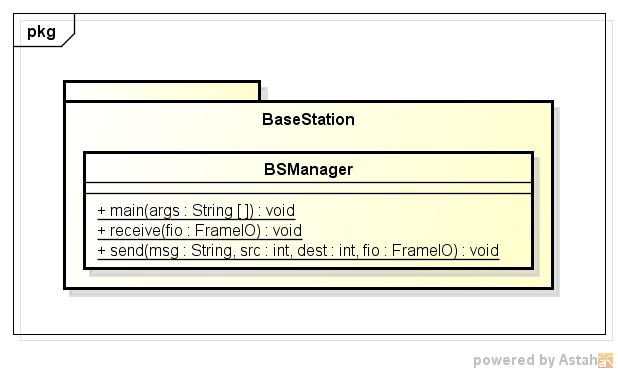
\includegraphics[scale=0.5]{KelasDiagramSederhana/BaseStation}  
	\caption[Kelas Diagram Sederhana Pada Aplikasi di BaseStation]{Kelas Diagram Sederhana Pada Aplikasi di BaseStation} 
	\label{fig:BaseStation} 
\end{figure} 

Keterangan Package BaseStation:
\begin{itemize}
	\item Kelas BSManager : Kelas ini digunakan untuk sebagai main class dari package ini. Kelas ini akan berfungsi untuk menerima pesan dari sensor node, menerima perintah dari UserApp, dan mengirim perintah ke sensor node. Metode yang bertugas untuk mengirim pesan adalah metode {\it send()} dan Metode {\it receive()} berfungsi untuk menerima pesan.
\end{itemize}

\begin{figure} [H]
	\centering  
	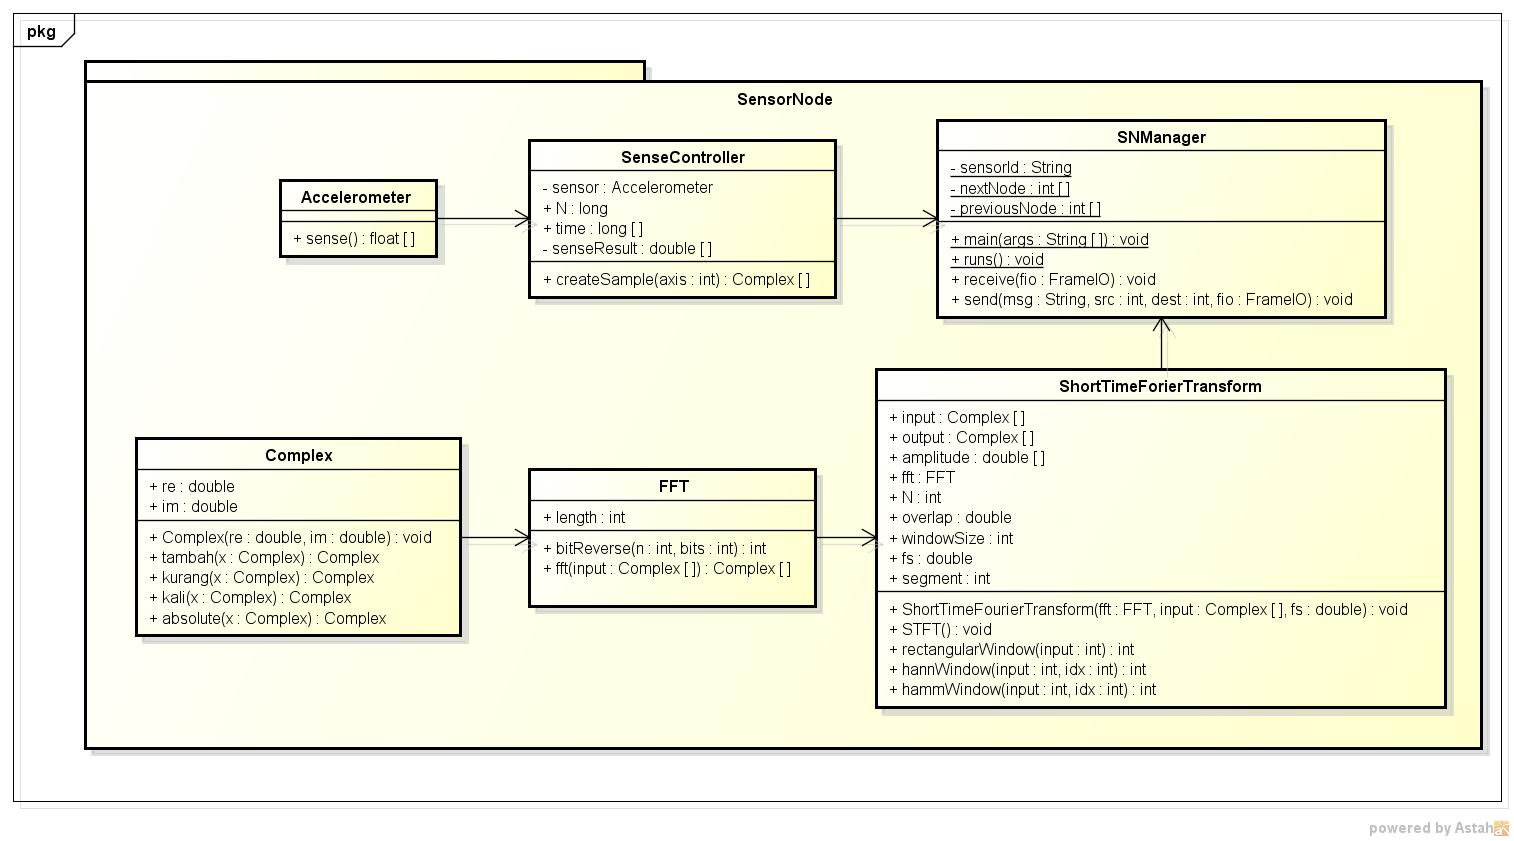
\includegraphics[scale=0.3]{KelasDiagramSederhana/SensorNode}  
	\caption[Kelas Diagram Sederhana Pada Aplikasi di SensorNode]{Kelas Diagram Sederhana Pada Aplikasi di SensorNode} 
	\label{fig:SensorNode} 
\end{figure} 

\newpage
Keterangan Package SensorNode:
\begin{itemize}
	\item Kelas Accelerometer : Kelas ini digunakan untuk menginisialisasi akselerometer pada sensor node. Untuk melakukan {\it sensing} digunakan metode {\it sense()}.
	\item Kelas SenseController : Kelas ini digunakan untuk mengatur pengukuran getaran dan membuat {\it sample} getaran. Terdapat atribut {\it N} sebagai panjang {\it sample}, {\it time} untuk menyimpan waktu saat {\it sensing}, dan {\it senseResult} untuk menyimpan hasil {\it sensing}. Metode {\it createSample()} pada kelas ini digunakan untuk membuat {\it sample}.
	\item Kelas Complex : Kelas ini merepresentasikan bilangan kompleks. Terdapat atribut {\it re} untuk menyimpan bilangan riil dan {\it im} untuk menyimpan bilangan imajiner. Metode {\it tambah()}, {\it kurang()}, {\it kali()}, dan {\it absolute()} digunakan untuk operasi bilangan {\it Complex}.
	\item Kelas FFT : Kelas ini berisi implementasi dari algoritma FFT. Terdapat atribut {\it length} untuk menyimpan panjang dari FFT. Metode {\it bitReverse()} dan {\it fft()} sebagai implementasi dari algoritma FFT.
	\item Kelas ShortTimeFourierTransform : Kelas ini berisi implementasi dari algoritma STFT. Atribut {\it input} untuk menyimpan hasil {\it sensing}, {\it output} untuk menyimpan hasil dari STFT , {\it amplitude} untuk menyimpan hasil amplitude dari {\it output}, {\it fft} sebagai objek dari FFT yang digunakan, {\it N} sebagai panjang dari STFT, {\it overlap} untuk menyimpan nilai {\it overlap}, {\it windowSize} untuk menyimpan panjang dari {\it window} yang digunakan, {\it fs} untuk menyimpan nilai dari {\it sampling rate}, dan {\it segment} untuk menyimpan besar {\it segment} yang digunakan. Terdapat 3 metode untuk {\it window function} dari STFT, yaitu {\it rectangularWindow()}, {\it hannWindow}, dan {\it hammWindow}. Metode {\it STFT()} sebagai implementasi dari algoritma STFT.
	\item Kelas SNManager : Kelas ini menjadi main class dari package ini dan digunakan untuk menerima dan mengirim pesan /  hasil ekstraksi fitur ke sensor node / {\it base station}. Atribut {\it sensorId} untuk menyimpan id dari sensor, {\it nextNode} untuk menyimpan node - node selanjutnya, dan {\it previousNode} untuk menyimpan node - node sebelumnya. Metode {\it send()} untuk mengirim pesan ke sensor node lain, {\it receive()} untuk menerima pesan dari sensor node lain, dan {\it runs()} untuk melakukan insialisasi.
\end{itemize}

\begin{figure} [H]
	\centering  
	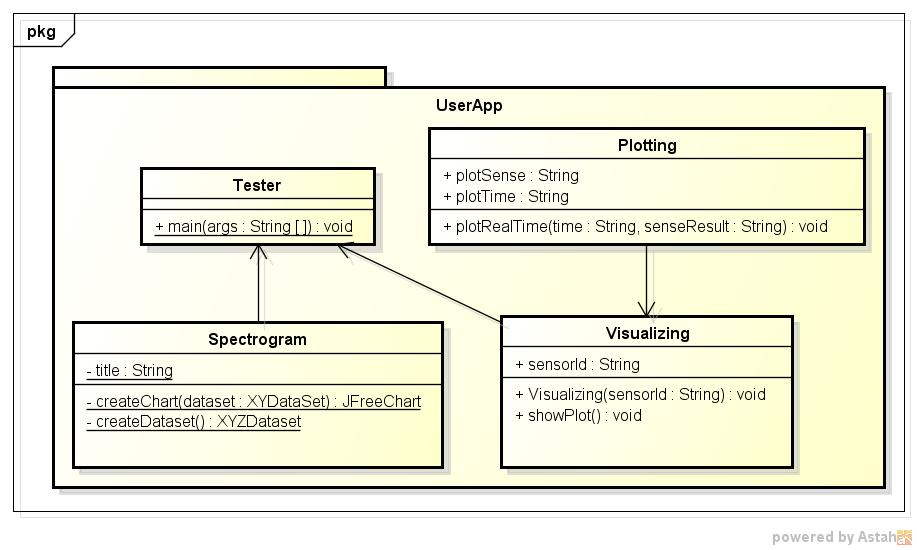
\includegraphics[scale=0.45]{KelasDiagramSederhana/UserApp}  
	\caption[Kelas Diagram Sederhana Pada Aplikasi di UserApp]{Kelas Diagram Sederhana Pada Aplikasi di UserApp} 
	\label{fig:UserApp} 
\end{figure} 

Keterangan Package UserApp:
\begin{itemize}
	\item Kelas Tester : Kelas ini digunakan sebagai main class yang menerima input dari pengguna dan menampilkan output ke pengguna.
	\item Kelas Visualizing : Kelas ini bertugas untuk membuat tampilan visualisasi dari hasil {\it sensing}. Terdapat atribut {\it sensorId} untuk menyimpan sensorId dan metode {\it showPlot()} untuk menampilkan grafik.
	\item Kelas Plotting : Kelas ini bertugas untuk membantu kelas Visualizing dalam membuat plot dari hasil {\it sensing}. Terdapat atribut {\it plotSense} untuk menyimpan hasil {\it sensing} untuk di plot dan {\it plotTime} untuk menyimpan waktu saat {\it sensing} untuk di plot. Metode {\it plotRealtime()} digunakan untuk menampilkan plot pada grafik di kelas Visualizing.
	\item Kelas Spectrogram : Kelas ini digunakan untuk menampilkan grafik spectrogram dari hasil ekstraksi fitur. Terdapat atribut {\it title} untuk menyimpan judul spectrogram dan metode {\it createDataset()} untuk membuat {\it data set} dari hasil ekstraksi fitur dan {\it createChart()} untuk membuat grafik.
\end{itemize}


\section{Analisis Proses Ekstraksi Fitur}
\label{sec:analisisProses}
Pada subbab ini akan dijelaskan mengenai proses ekstraksi fitur dari hasil pengukuran akselerometer. 

\subsection{Analisis {\it Sample} Data Akselerometer}
\label{subsec:sample}
{\it Sample} data akselerometer yang digunakan untuk ekstraksi fitur diambil dari hasil pengukuran salah satu sumbu akselerometer ($x$/$y$/$z$) (\ref{subsec:akselerometer}). {\it Sample} yang dibuat harus berkelipatan 2 (\ref{subsec:fft}). Pada pembuatan {\it sample} disimpan waktu setiap kali pengukuran dilakukan. Setelah pembuatan {\it sample} dihitung {\it sampling rate} dari pembuatan sample dengan membagi jumlah {\it sample} dengan waktu yang dibutuhkan untuk membuat {\it sample}.

\subsection{Analisis Algoritma {\it Short Time Fourier Transform}}
Proses STFT ini adalah ekstraksi fitur data akselerometer dari domain waktu ke domain frekuensi yang dicuplik sebesar {\it sample}(\ref{subsec:stft}). Besar {\it window} yang digunakan untuk STFT ini adalah setengah panjang {\it sample}. Seperti yang sudah dibahas pada Subbab \ref{subsec:stft}, Algoritma STFT menggunakan algoritma FFT untuk perhitungannya. Algoritma FFT yang akan digunakan untuk aplikasi ini adalah {\it Cooley-Tukey Algorithm}. Algoritma ini memerlukan jumlah {\it sample} $N$ berkelipatan 2 (\ref{subsec:sample}). {\it Sample} untuk algoritma ini harus berupa bilangan kompleks (\ref{subsec:dft}). Dalam membuat {\it sample} yang adalah bilangan real menjadi bilangan kompleks, maka {\it sample} dikonversi menjadi bilangan kompleks dengan memasukkan setiap nilai {\it sample} pada komponen real dan 0 pada komponen imajiner untuk setiap {\it sample} (\ref{subsec:complex}). Setelah dikonversi, {\it sample} akan diekstraksi fitur dengan {\it Rectangle window} (\ref{eqn:rectW}) / {\it Hanning window} / {\it Hamming window} dengan besar setengah dari {\it sample} dan nilai {\it overlap} sebesar 0\%. Dari besar {\it sample},besar {\it window}, dan nilai {\it overlap} dapat dihitung besar {\it segment}. 

\newpage
Hasil dari STFT adalah berupa matrix dengan panjang kolom sebesar panjang sample dan panjang baris sebesar {\it segment}. Isi dari matrix adalah hasil komputasi FFT dari waktu {\it segment}. Setiap {\it segment} pada matrix dikomputasi untuk mendapatkan {\it amplitude}(\ref{eqn:complexNumberMag}). Setiap {\it amplitude} yang diperoleh akan diplot pada grafik spectrogram dengan frekuensi dan waktu. 

Berikut pseudocode dari algoritma STFT secara sederhana.
\begin{algorithm}[htbp]
\label{stftSederhana}
		\caption{pseudocode {\it STFT()} sederhana}
		\begin{algorithmic}[1]
		\Function{STFT}{}
			\While {segment masih ada}
				\State {\it window} {\it sample} dengan {\it window function} berdasarkan besar {\it window} dan {\it overlap}
				\State Isi nilai 0 pada {\it sample} yang belum di {\it window}
				\State Komputasi {\it sample} yang sudah di {\it window} dengan algoritma FFT
				\State Hitung nilai {\it amplitude} dari setiap hasil FFT
			\EndWhile
		\EndFunction
	\end{algorithmic}
	\end{algorithm} 



